\documentclass[12pt]{article}
\usepackage{natbib}
\usepackage{graphicx} 
\usepackage{amsmath}
\bibliographystyle{plain}
% Increase margins (manually) 
  % Sides (odd- and even-numbered pages)
    \addtolength{\oddsidemargin}{-0.875in}
    \addtolength{\evensidemargin}{-0.875in}
    \addtolength{\textwidth}{1.75in}
  % Top/bottom
    \addtolength{\topmargin}{-0.875in}
    \addtolength{\textheight}{1.75in}
\title{ASTR 565 \\
Computer Problem 3: Convection and Radiation Zones in Main Sequence
Stars}
\author{Laurel Farris}
\date{03 November 2015}
\begin{document}
\maketitle

\section{Introduction}


% 1. 
% Make HR diagram
An HR diagram for all the stars is shown in figure \ref{hrdiagram}!

\begin{figure}%[h]
  \centering
  \includegraphics[width=7.0in]{hrdiagram.png}
  \caption{This plot shows...}
  \label{hrdiagram}
\end{figure}


\section{Methods}

% 2. Money plot!
%    Put this on a full page by itself, and e-mail the plot by itself.
\begin{figure}%[h]
  \centering
  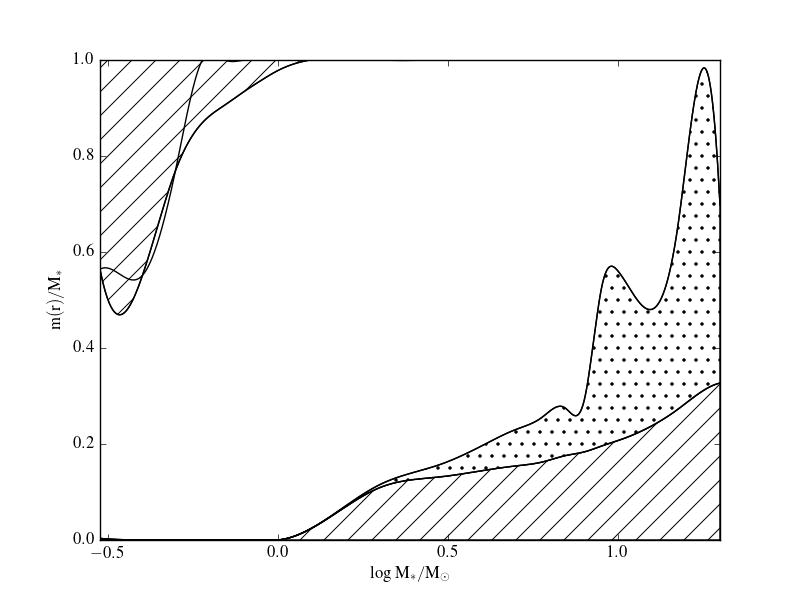
\includegraphics[width=7.0in]{money.png}
  \caption{This plot shows...}
  \label{money}
\end{figure}

% 3. Money plot again!
\begin{figure}%[h]
  \centering
  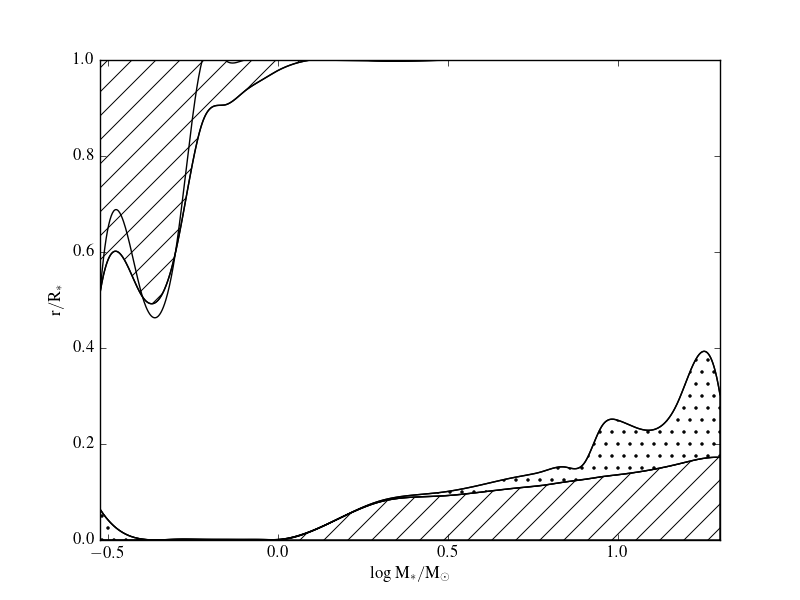
\includegraphics[width=7.0in]{money2.png}
  \caption{This plot shows...}
  \label{money2}
\end{figure}

% 4. 
% Write a couple paragraphs:
%  --> WHAT you did.
% How did you obtain the parameters in your plot? 
% In other words, how did you determine where the zones are from the
% stellar profiles?

% 5.
% four more plots! 2 for each of 2 models, one > 3Mo and one < 1.1 Mo

% 6.
% A PAGE OR TWO on the above four plots!!!!!
% What is happening?
% Connect what you see in these figs to the findings in the money plot
% Compare and contrast the behavior for the two different masses
% Describe and decipher any 'unusual' features you see, such as 
%   bumps or spikes, in each case.
% Connect to things we may have DISCUSSED IN CLASS, eg opacities.
% (more plots?)
% Question --> In the interior regions where del is large, what is
% your idea as to the physical reasons causing this?
%     (use equation 3.65 as a guide).
% Be thorough

\section{Results}


\section{Conclusions}
See the work these guys did \cite{Alongi}.

\newpage

\bibliography{reffile}
\end{document}


